\documentclass[conference]{IEEEtran}
\IEEEoverridecommandlockouts
\usepackage[font=footnotesize]{caption}
\usepackage{subcaption}
\usepackage{xcolor}
\usepackage[colorlinks]{hyperref}
\usepackage{fancyvrb}
\usepackage{tikz}
\usepackage{booktabs}

\newcommand*{\priority}[1]{\begin{tikzpicture}[scale=0.12]%
   \draw (0,0) circle (1);
   \fill[fill opacity=1,fill=black] (0,0) -- (90:1) arc (90:90-#1*3.6:1) -- cycle;
   \end{tikzpicture}}
\newcommand*{\priorityc}[1]{
\resizebox{0.8em}{0.8em}{
 {\protect\tikz{ \protect
   \draw[line width=1mm, black] (0,0) circle (1); \fill[fill opacity=1,fill=black] (0,0) -- (90:1) arc (90:90-#1*3.6:1) -- cycle;
   } }}}
%
\definecolor{kvdclr}{rgb}{0.3,0.0,0.8}
\DefineVerbatimEnvironment{thegamma}{Verbatim}{fontfamily=zi4,numbers=left,xleftmargin=6mm,fontsize=\small,commandchars=\\\{\}}
\newcommand{\kvd}[1]{\textbf{#1}}
\newcommand{\ikvd}[1]{{\fontfamily{zi4}\selectfont\small #1}}

\begin{document}
\title{\textbf{The Gamma}: Programmatic Data\\ Exploration for Non-programmers}
\author{\IEEEauthorblockN{Tomas Petricek}
\IEEEauthorblockA{University of Kent, UK and Charles University, Czech Republic \\
\texttt{tomas@tomasp.net}}}

\maketitle

\begin{abstract}
Data exploration tools based on code can access any data source, result in reproducible scripts and
encourage users to verify, reuse and modify existing code. Unfortunately, they are hard to use and
require expert coding skills. Can we make data exploration tools based on code accessible to non-experts?

We present The Gamma, a novel text-based data exploration environment that answers the question in
the affirmative. The Gamma takes the idea of code completion to the limit. Users create transparent
and reproducible scripts without writing code, by repeatedly choosing from offered code completions.

The Gamma is motivated by the needs of data journalists and shows that we may not need to shy away
from code for building accessible, reproducible and transparent tools that allow a broad public to
benefit from the rise of open data.
\end{abstract}

\begin{IEEEkeywords}
data exploration, data journalism
\end{IEEEkeywords}
\IEEEpubid{978-1-6654-4214-5/22/\$31.00 \copyright 2022 IEEE}
\IEEEpubidadjcol

% ==================================================================================================

\section{Introduction}
\noindent
Despite the advances on visual tooling, programmatic data exploration remains the choice of
expert analysts. It is flexibile, offers greater reusability and leads to transparent
analyses. The design of a programmatic data exploration tool that would be accessible to data
journalists poses a number of design challenges. First, the tool needs to have a low barrier to
entry to support first-time users without training. Second, it needs to support multiple
data sources in a uniform way to allow transfer of knowledge across domains. Finally, users need
to be able to learn by looking at existing data analyses.

We present The Gamma, a text-based data exploration tool for non-experts that is based on a single,
easy to understand interaction principle. It provides a uniform access to data tables, graph
databases and data cubes and leads to transparent analyses that can be easily reproduced,
encouraging learning and critical engagement with data.

The Gamma is based on \emph{iterative prompting}, which turns code completion from a programmer
assistance tool into a non-expert programming mechanism that allows users to construct all valid
data exploration scripts just by repeatedly choosing an item from a list of offered options.
The design favors \emph{recognition over recall} and allows non-programmers to construct entire
scripts without first learning to code. Yet, the result remains a transparent and reproducible script.
A crucial feature is that iterative prompting only offers operations that are valid in a given
context and that it offers all such operations; it is both correct and complete.

The Gamma focuses on tasks that a data journalist may want to complete (Figure~\ref{fig:thegamma}).
The user accesses data available in a structured format. They make several experiments to find an
interesting insight, e.g.~by applying different aggregations or filters. They
visualize the results using a table or a chart before publishing their analysis. The
Gamma makes such programmatic data exploration simple enough for non-programmers. Scraping and
cleaning of messy data or building custom data visualizations is outside of the scope of
our work, but exposing such functionality using iterative prompting is an interesting and
worthwhile future challenge.

\begin{figure}
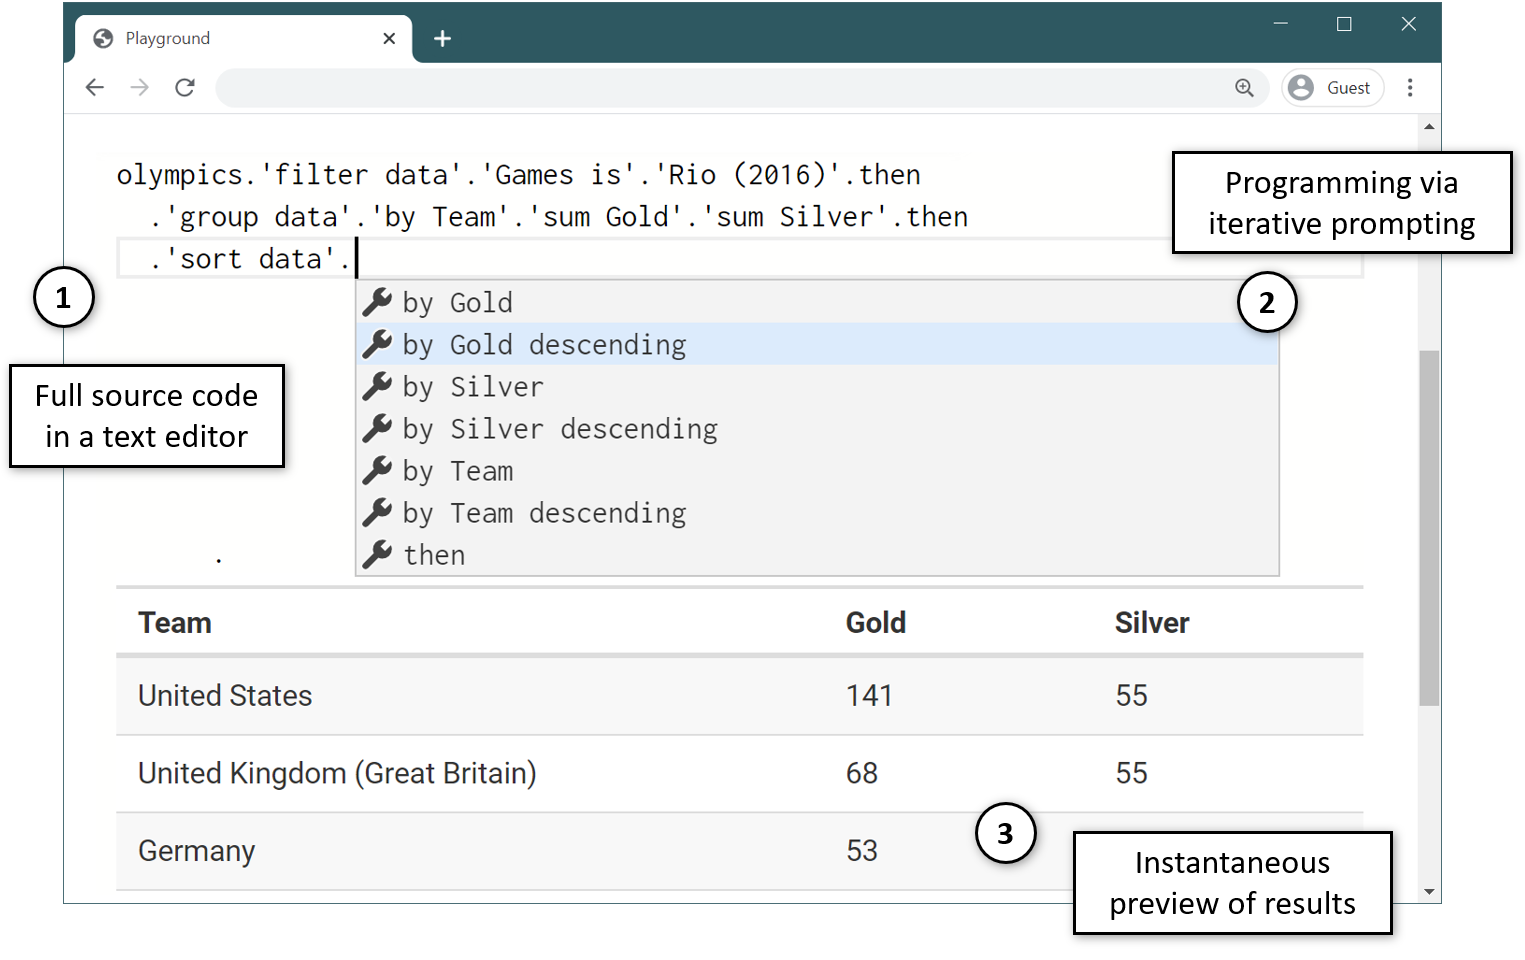
\includegraphics[width=1\columnwidth]{figures/thegamma-annot}
\caption{Obtaining teams with the greatest number of gold medals from Rio 2016
Olympics: (1) Reproducible The Gamma script; (2) contextual iterative prompting
offering ways of sorting the data; (3) an instant preview of results.}
\label{fig:thegamma}
\vspace{-1em}
\end{figure}

\IEEEpubidadjcol
In this paper, we describe and evaluate the design principles behind The Gamma project:

\begin{itemize}
\setlength\itemsep{0.25em}
\item We introduce the iterative prompting principle in The Gamma (Section~\ref{sec:overview})
  and show how it can be used for querying of distinct data sources including data tables, graph
  databases and data cubes (Section~\ref{sec:system}).

\item We illustrate the expressiveness of the system through a case study (Section~\ref{sec:cases})
  and evaluate it through a user study (Section~\ref{sec:study}), confirming that non-programmers
  can use The Gamma to construct non-trivial data queries.

\item We reflect how our design lowers barriers to entry, supports learning without experts and offers a
  complete and correct program construction method (Section~\ref{sec:discuss}).
\end{itemize}

\noindent
The Gamma is available at \url{http://thegamma.net},
both as an open-source library and a hosted data exploration service.

% ==================================================================================================

\section{Related Work}
\noindent
We aim to make recent advances on information-rich programming~\cite{inforich} available to
non-programmers~\cite{enduser,smallmatter}, in the context of data journalism~\cite{ddj}.
Our work features a novel combination of characteristics in that our iterative prompting
interaction principle is centered around code, but reduces the conceptual complexity of coding to
a single basic kind of interaction.

\vspace{0.5em}
\subsubsection*{Code Completion for Data Science}

The Gamma utilizes type providers~\cite{inforich,fsdata}, which integrate external data into a
static type system. This enables auto-completion~\cite{assistants}, which we turn into a tool for
non-programmers. Similar systems based on machine learning and domain specific
languages~\cite{predictive,proactive} do not guarantee completeness, i.e.~it is unclear whether the user
can create all possible scripts. Approaches based on natural language are
effective~\cite{eviza,codemend,iris}, but hide the underlying structure and do not help users understand
the exact operations performed. Code completion based on machine learning~\cite{mlcomplete,statcomplete}
also exists for general-purpose programming languages used by data scientists such as
Python~\cite{pythia}, but this focuses on providing assistance to expert programmers.

\vspace{0.5em}
\subsubsection*{Notebooks and Business Intelligence Tools}

Notebooks such as Jupyter~\cite{jupyter} are widely used data exploration environments for
programmers. The Gamma targets non-experts, but could be integrated with a multi-language
notebook system~\cite{wrattler}.
%
Spreadsheets, business intelligence~\cite{tableau,powerbi} and other visual data analytics
tools~\cite{control,vizdom} do not involve programming, but require mastering a complex GUI.
In contrast, in The Gamma, all operations can be completed through a single kind of interaction.
Several systems~\cite{potter,wrangler,lyra} record interactions with the GUI as a script that can
be modified by the user. Unlike in The Gamma, the generated code does not guide the user in
learning how to use the system.

\vspace{0.5em}
\subsubsection*{Easier Programming Tools}
Many systems aim to make programming easier. Victor~\cite{principle} inspired work on live
environments environments~\cite{review,liveroad,lighttable} that help programmers understand how
code relates to output; exploratory systems~\cite{variolite,exploratory} assist with completing
open-ended tasks; and system combining code with visualization also exists for graph
querying~\cite{guess}. The Gamma is live in that our editor gives an instant preview of the results.
To avoid difficulties with editing code as text, some systems use structured
editors~\cite{structure-based,livenut,lamdu,subtext,directprog}. Many systems simplify programming by
offering high-level abstractions, e.g.~for interactive news articles~\cite{idyll}, statistical
analyses~\cite{tea}, data visualization~\cite{interactionviz,vegalite}. The Gamma
provides high-level abstractions for data querying, but supporting other tasks remains future work.

\vspace{0.5em}
\subsubsection*{Programming without Writing Code}
In programming by example~\cite{byexample}, used for example in spreadsheets~\cite{spreadsheetpbe,flashextract},
the user gives examples of desired results. In direct manipulation~\cite{direct}, a program is
specified by interacting with the output. This has been used in the visual domain~\cite{sketchnsketch}, but also for data
querying~\cite{dynamicq,vlang,visage}. Direct manipulation can also support data exploration by letting
users partially edit queries,~e.g. by changing quantifiers as in DataPlay~\cite{dataplay}.


% ==================================================================================================

\section{Overview}
\label{sec:overview}

\noindent
The Gamma is a text-based system that allows non-experts to explore data using
iterative prompting -- by repeatedly selecting an item from an auto-complete list. The study
presented in Section~\ref{sec:study} confirms that the kind of data exploration shown in the next
section can be successfully done by non-experts.

We introduce The Gamma by walking through a
typical data exploration task. A data journalist from Kent is exploring travel expense claims
by members of the House of Lords published by the UK government \cite{lords}. After importing
the CSV file through a web interface, the environment is initialized with code that refers
to the imported data as \ikvd{expenses} using the type provider for tabular data (Section~\ref{sec:system}).
The journalist types `.' (dot) to start exploring the data:

\vspace{0.5em}
\begin{thegamma}
expenses.
\end{thegamma}
\qquad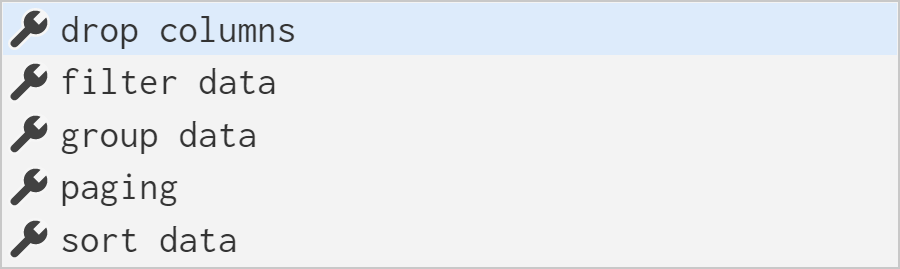
\includegraphics[width=0.7\columnwidth]{figures/lords0}
\vspace{0.5em}

\noindent
The type provider offers a list of operations that the journalist can perform. To find House of Lords
members from Kent, the journalist chooses \ikvd{filter data}. She is then offered a list of columns
based on the schema of the CSV file and chooses \ikvd{County is}. The completion lists
counties in the data set:

\vspace{0.5em}
\begin{thegamma}
expenses.'filter data'.'County is'.
\end{thegamma}
\qquad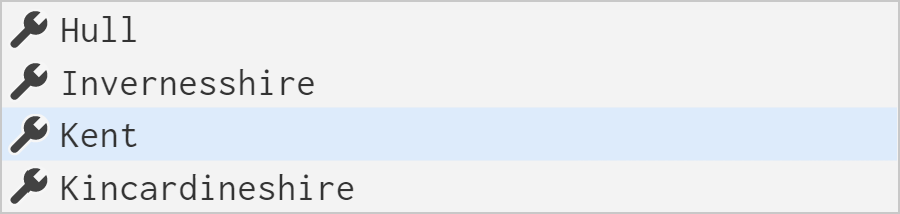
\includegraphics[width=0.7\columnwidth]{figures/lords1}
\vspace{0.5em}

\noindent
The journalist chooses Kent. The Gamma evaluates the code on-the-fly and shows a
preview of results.

\vspace{0.5em}
\begin{thegamma}
expenses.'filter data'.'County is'.Kent
\end{thegamma}
\vspace{0.4em}\qquad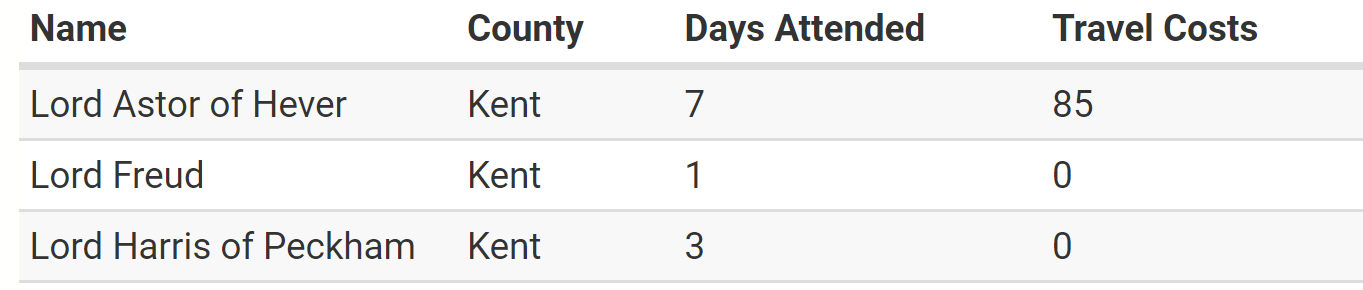
\includegraphics[width=0.95\columnwidth]{figures/lords2}
\vspace{0.5em}

\noindent
The journalist decides to compare travel costs. She finishes specifying the
filtering condition by choosing \ikvd{then} and is offered the same list of querying operations as
in the first step. She selects  \ikvd{sort data} and is offered a list of sorting options:

\vspace{0.5em}
\begin{thegamma}
expenses.'filter data'.'County is'.Kent.then.
  'sort data'.
\end{thegamma}
\qquad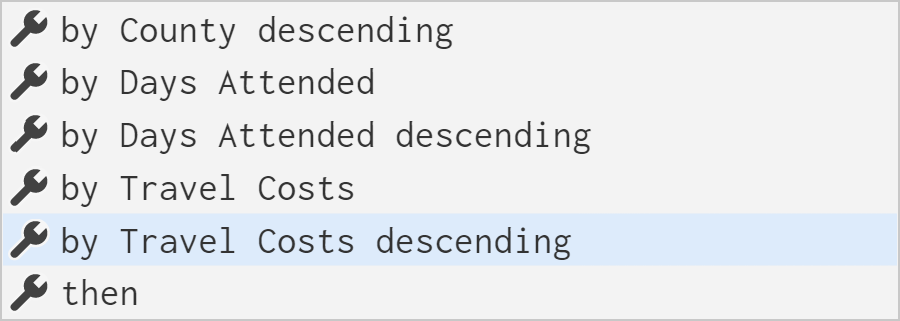
\includegraphics[width=0.7\columnwidth]{figures/lords3}
\vspace{0.5em}

\noindent
The journalist chooses \ikvd{then} and is, again, offered the list of querying operation. She
uses \ikvd{paging} to get the top 4 records, which requires typing \ikvd{4} as the argument.
She then uses the \ikvd{get series} operation to obtain a data series associating travel
expenses with a name, which is automatically visualized:

\vspace{0.5em}
\begin{thegamma}
expenses.'filter data'.'County is'.Kent.then
  .'sort data'.'by Travel Costs descending'.then
  .paging.take(4).'get series'
    .'with key Name'.'and value Travel Costs'
\end{thegamma}
\vspace{0.2em}\quad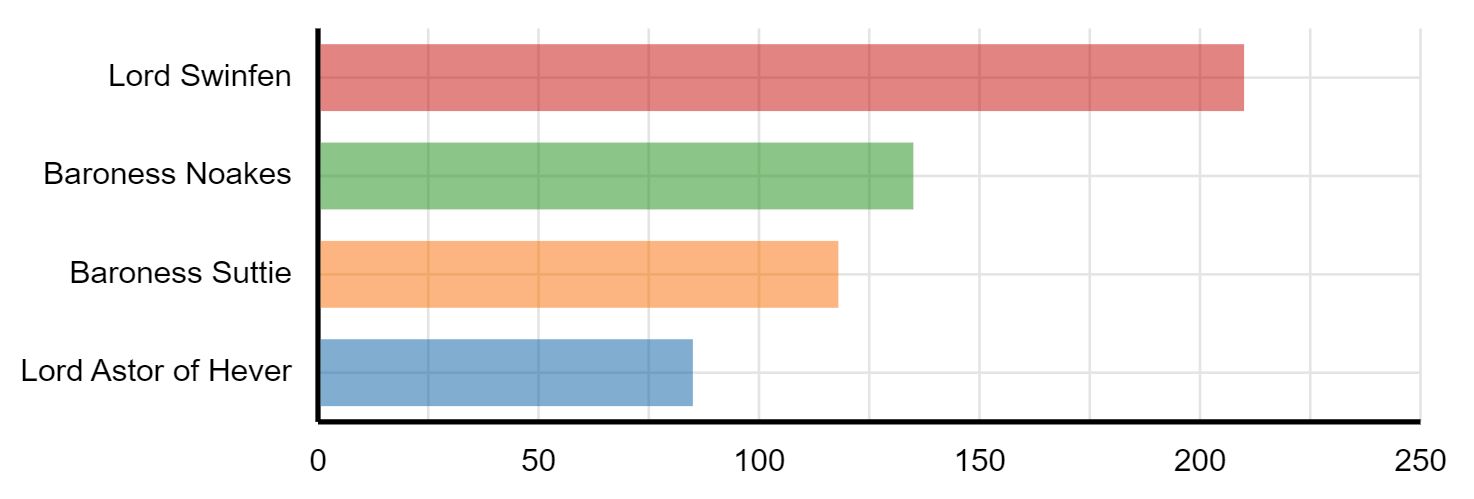
\includegraphics[width=0.95\columnwidth]{figures/lords4}

The code is not unlike an SQL query, except that the whole script is constructed using
iterative prompting, by repeatedly selecting one of the offered members. Those represent both
operations, such as \ikvd{sort by} and arguments, such as \ikvd{Kent}. The only exception
is when the analyst needs to type the number \ikvd{4} to specify the number of items to take.

\section{System description}
\label{sec:system}

\noindent
A program in The Gamma is a sequence of commands that can be either a variable declarations or
an expression that evaluates to a value. An expression is a reference to a data source followed
by a chain of member accesses. Each expression has a type that is used to generate options in
auto-completion. A type defines a list of members that, in turn, have their own types.
The types are not built-in, but are generated by type providers for individual data sources.
The syntax and semantics of the language has been described elsewhere \cite{tglive}.

A new data source can be supported by implementing a \emph{type provider},
which defines a domain specific language for exploring data of a particular kind.
A type provider generates object types with members (such as \ikvd{paging} or \ikvd{Kent})
that are accessed via iterative prompting. We outline type providers for exploring data cubes
(inspired by Syme et al. \cite{inforich}), tabular data (formalized elsewhere \cite{dotdriven}), and graph databases.

\vspace{0.5em}
\subsubsection*{Data Cube Provider}
Data cubes are multi-dimensional arrays of values. For example, the World Bank collects a range of
indicators about many countries each year while the UK government expenditure records spending for
different government services, over time, with different adjustments:

\vspace{0.25em}
\begin{thegamma}
worldbank.byCountry.'United States'.
  'Climate Change'.'CO2 emissions (kt)'

expenditure.byService.Defence.inTermsOf.GDP
\end{thegamma}
\vspace{0.25em}

\noindent
The dimensions of the \ikvd{worldbank} cube are countries, years and indicators, whereas the dimensions
of \ikvd{expenditure} are government services, years and value type (adjusted, nominal,
per GDP).  Figure~\ref{fig:cubetp} illustrates how the provider allows users to slice the data cube.
Choosing \ikvd{byCountry.\textquotesingle United States\textquotesingle},
restricts the cube to a plane and \ikvd{\textquotesingle CO2 emissions (kt)\textquotesingle}
then gives a series with years as keys and emission data as values. Similarly, we could first filter the
data by a year or an indicator. The same mechanism is used to select UK government spending on
defence in terms of GDP.
%  As there is no widely used standard format for data cubes, adding another data cube to The Gamma
% currently requires implementing a new type provider.

\vspace{0.5em}
\subsubsection*{Graph Database Type Provider}
Graph databases store nodes representing entities and relationships between them.
The following example explores a database of Doctor Who characters and episodes. It retrieves
all enemies of the Doctor that appear in the Day of the Moon episode:

\vspace{0.25em}
\begin{thegamma}
drwho.Character.Doctor.'ENEMY OF'.'[any]'
  .'APPEARED IN'.'Day of the Moon'
\end{thegamma}
\vspace{0.25em}

\noindent
We start from the \ikvd{Doctor} node and then follow two relationships. We use
\ikvd{\textquotesingle ENEMY OF\textquotesingle.\textquotesingle [any]\textquotesingle}
to follow links to all enemies of the Doctor and then specify
\ikvd{\textquotesingle APPEARED IN\textquotesingle}
to select only enemies that appear in a specific episode. The query is illustrated in
in Figure~\ref{fig:graphtp}. The members are generated from the data;
\ikvd{ENEMY OF} and \ikvd{APPEARED IN} are labels
of relations and \ikvd{Doctor} and \ikvd{Day of the Moon} are labels of nodes. The
\ikvd{[any]} member defines a placeholder that can be filled with any node with the specified
relationships. The results returned by the provider is a table of properties of all nodes
along the specified path, which can be further queried and visualized.

\vspace{0.5em}
\subsubsection*{Tabular Data Provider}

Unlike the graph and data cube providers, the type provider for tabular data does not just
allow selecting a subset of the data, but it can be used to construct SQL-like query. Consider
the example of querying expense claims from Section~\ref{sec:overview}, which filters and then
sorts the data.

When using the provider, the user specifies a sequence of operations. Members such as
\ikvd{\textquotesingle filter data\textquotesingle} or \ikvd{\textquotesingle sort data\textquotesingle}
determine the operation type. Those are followed by members that specify operation parameters.
For example, when filtering data, we first select the column and then choose a desired value.
Unlike SQL, the provider only allows users to choose from pre-defined filtering conditions,
but this is sufficient for constructing a range of practical queries.

\begin{figure}[h]
\centering
\begin{subfigure}[b]{0.5\textwidth}
  \centering
  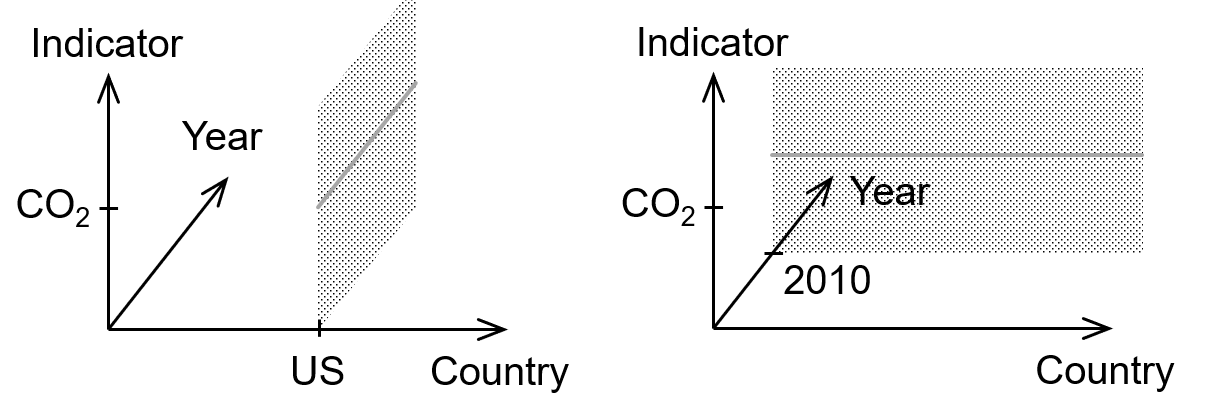
\includegraphics[scale=0.27]{figures/cubetp}
  \vspace{0.5em}
  \caption{Exploring World Bank data using the data cube type provider, users
    choose values from two dimensions to obtain a data series.}
  \label{fig:cubetp}
  \vspace{1em}
\end{subfigure}
\begin{subfigure}[b]{0.45\textwidth}
  \centering
  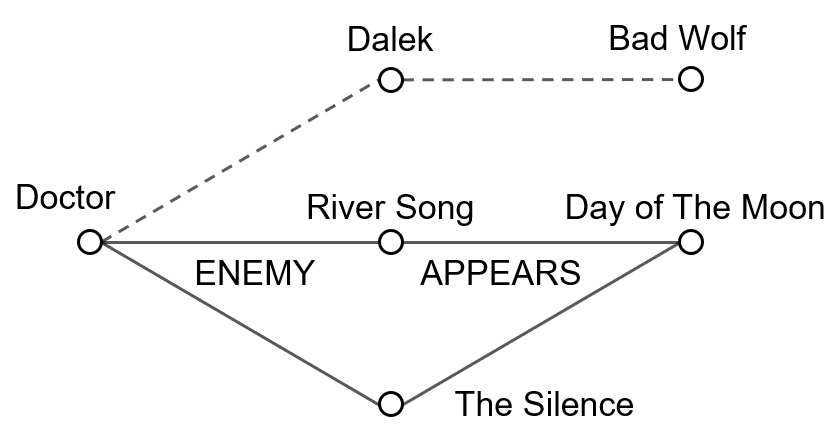
\includegraphics[scale=0.31]{figures/graphtp}
  \caption{To query graph data, the user specifies a path through the data, possibly with
    placeholders to select multiple nodes.}
  \label{fig:graphtp}
  \vspace{0.5em}
\end{subfigure}
\caption{Type providers for exploring cube and graph data.}
\label{fig:tps}
\vspace{-0.5em}
\end{figure}


% ==================================================================================================

\section{Case Study}
\label{sec:cases}

\noindent
The Gamma aims to simplify programmatic data exploration while keeping enough expressive power
to allow users to create interesting data explorations. To show what can be achieved by
interactive prompting, we present a case study that explores a graph database with Dr Who
series data.\footnote{See: \url{http://gallery.thegamma.net/87/}. We also used The Gamma for
projects exploring the UK government expenditure, activities of a research institute and Olympic
medal winners, available at \url{http://turing.thegamma.net} and \url{http://rio2016.thegamma.net}}.

The following constructs a chart (Figure~\ref{fig:cases-dr}) of top Dr Who villains by the number of
episodes in which they appear. This case is interesting as it combines the graph database provider
for fetching the data with the tabular data provider:

\vspace{0.25em}
\begin{thegamma}
drWho.Character.Doctor.'ENEMY OF'.'[any]'
     .'APPEARED IN'.'[any]'.explore
  .'group data'.'by Character name'
     .'count distinct Episode name'.then
  .'sort data'.'by Episode name descending'.then
  .paging.take(8).'get series'
     .'with key Character name'
     .'and value Episode name'
\end{thegamma}
\vspace{0.25em}

\noindent
Line 1 use the graph provider to find all paths linking the Doctor with any
character linked via \ikvd{ENEMY OF}, followed by any episode linked by \ikvd{APPEARED IN}.
This produces a table that can be analysed using the tabular data provider by selecting
\ikvd{explore}. For each character (the villain) we count the number of
distinct episodes. The result is shown in Figure~\ref{fig:cases-dr}.
Despite performing a sophisticated data analysis that involves a graph database query,
followed by an SQL-like data aggregation, the code can be constructed using iterative
prompting, with the exception of the numbers in paging.

% ==================================================================================================

% TODO Study improvements
% - The questionaire needs a bit more introduction when you present  the study.
% - When looking at the data for the questionaire, it seems somewhat inconclusive
%    as all the values lie around 2.5.  I think this warrants a bit more discussion.
% - Connected to this, I would recommend to highlight the successes of the study a bit more in the
%     discussion and  presentation of the results. You actually got non-programmers to do
%     sophisticated queries! That you didn't get support for all RQs is perhaps more a result of being quite  ambitious!


% \begin{table*}
% \vspace{-0.5em}
% \centering
% \renewcommand{\arraystretch}{1.25}
% \begin{tabular}{l l l c l}
%   \toprule
%     & {\small \textit{Task}}
%     & {\small \textit{Kind}} & {\small \textit{Done}}
%     & {\small \textit{Notes}} \\
%   \midrule
%   \small \#1\qquad\qquad & \small expenditure \qquad\qquad & \small cube \qquad\qquad & \qquad\priority{50}\qquad\qquad & {\small Obtained one of two data series}\\
%   \small \#2 & \small expenditure & \small cube & \priority{100} & {\small Explored furhter data series independently}\\
%   \small \#3 & \small expenditure & \small cube & \priority{100}& {\small Explored further data series independently}\\
%   \small \#4 & \small expenditure & \small cube & \priority{75}& {\small Completed following a hint to use another member }\\
%   \small \#5 & \small expenditure & \small cube & \priority{100}& {\small Explored further data series independently}\\
%   \small \#6 & \small worldbank & \small cube & \priority{75} & {\small Completed after a syntax hint about whitespace}\\
%   \small \#7 & \small worldbank & \small cube & \priority{100} & {\small Completed very quickly }\\
%   \small \#8 & \small worldbank & \small cube & \priority{100} & {\small Completed, but needed longer to find correct data }\\
%   \small \#9 & \small lords & \small table & \priority{75} & {\small Struggled with composition of operations}\\
%   \small \#10 & \small lords & \small table & \priority{100} & {\small Completed very quickly }\\
%   \small \#11 & \small lords & \small table & \priority{75} & {\small With a hint to avoid operations taking  arguments}\\
%   \small \#12 & \small olympics & \small table & \priority{75}  & {\small With a hint to avoid operations taking arguments}\\
%   \small \#13 & \small olympics & \small table & \priority{75}  & {\small With hints about `then' and operations taking arguments}\\
%   \bottomrule
% \end{tabular}
%
% \caption{\centering Overview of work completed by individual participants in the study. \\The marks denote:
%  \priorityc{100} = completed, \priorityc{75} = required some guidance, \priorityc{50} = partially completed}
% \label{tab:tasks}
% \vspace{-0.5em}
% \end{table*}


\section{User Study}
\label{sec:study}

\noindent
Data exploration environments are complex systems that do not yield to simple controlled
experimentation~\cite{evaluating}. Rather than comparing our work with other tools, we
evaluate whether The Gamma can be successfully used by non-programmers.

\begin{figure}[t]
\centering
\vspace{-0.25em}
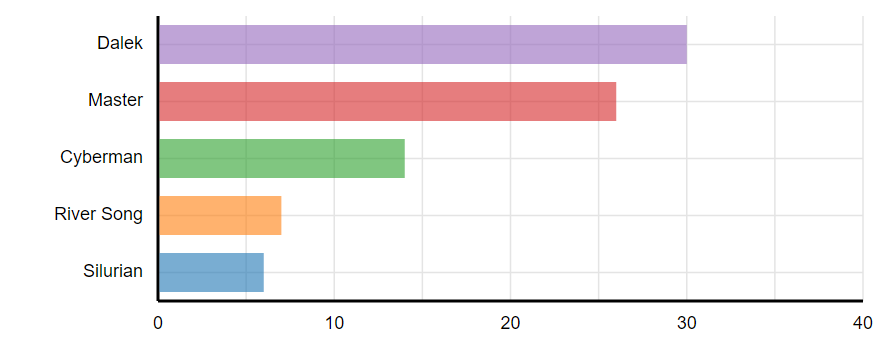
\includegraphics[width=0.95\columnwidth]{figures/cases-dr}
\vspace{-0.5em}
\caption{Who does the Dr Who fight most frequently?}
\label{fig:cases-dr}
\vspace{-1em}
\end{figure}


We performed a between-subjects study to assess whether non-programmers are able to complete a
simple data exploration task using The Gamma. We recruited 13 participants (5 male, 8 female)
from a business team of a research institute working in non-technical roles (project management,
communications). Only one participant (\#12) had prior programming experience.
%
We split participants into 4 groups and asked each group to complete a different task.
We gave participants a brief overview of The Gamma. The participants then worked for 30
minutes, after which we conducted a semi-structured group interview. We offered guidance
if participants were unable to progress for more than 5 minutes. The four tasks were:


\vspace{0.5em}
\begin{itemize}
\setlength\itemsep{0.5em}
\item \emph{Expenditure.} Participants were shown the \emph{worldbank} data cube
  and were asked to compare UK spending on `Public order and safety'' and ``Defence''
  using another data cube.
\item \emph{Lords.} Participants were shown \emph{worldbank} and were asked to use the
  \emph{expenses} data table provider to sort London House of Lords members by their
  travel costs.
\item \emph{Worldbank.} Participants were given a minimal iterative prompting demo and
  a code sample using \emph{worldbank}. They were asked to solve another \emph{worldbank} task.
\item \emph{Olympics.} Participants were given a demo using \emph{olympics} that did not involve grouping.
  They were asked to solve a problem involving grouping and aggregation.
\end{itemize}
\vspace{0.5em}

%
%Some aspects of the study aim to shed light on three questions concerning learnability
%of The Gamma, in particular whether knowledge can be trasferred between different data sources
%(\emph{RQ2a}), whether users can learn from code samples without a detailed guidance
%(\emph{RQ2b}) and to what extent they form a correct mental model of a more complex query
%language used in the tabular data source (\emph{RQ2c}).
%

%\vspace{0.5em}\noindent\emph{RQ2: Can knowledge transfer between data sources?}\hspace{0.3em}
%Our second hypothesis is that users familiar with the iterative prompting principle will be able to
%use an unfamiliar data source. We designed two of the four tasks to test this. Participants were
%shown a demo using one data source and then asked to complete a task using a different one.
%
%\vspace{0.5em}\noindent\emph{RQ3: Can users learn from just code samples?}\hspace{0.3em}
%Our third hypothesis is that users can learn through percolation, i.e.~by looking at the source
%code of published analyses. In one of our tasks, participants were given a minimal explanation
%of The Gamma (showing how to initiate the iterative prompting process) together with
%an extensive code sample.
%

\noindent
Our primary hypothesis was that non-programmers will be able to use The Gamma to explore
data. This was tested by all four tasks for one of the supported data sources.

The tasks \emph{expenditure} and \emph{lords} further test if knowledge can be transferred between
different data sources by using one sources in the introduction and another in the task;
\emph{worldbank} explores whether users can learn how to use a data source from just code samples;
and \emph{lords} lets us study to what extent participants form a correct mental model of the
more complex query language used in the tabular data source.


\vspace{0.5em}
\emph{Can non-programmers explore data with The Gamma?}~
All participants were able to complete, at least partially, a non-trivial data exploration task and
only half of them required further guidance. Participants spent 10--25 minutes (average 17)
working with The Gamma and 12 out of 13 completed the task; 6 required assistance, but 3 of those
faced the same issue related to operations taking arguments (discussed later).

A number of participants shared positive comments in the group interviews.
Participant \#3 noted that \emph{``this is actually pretty simple to use,''}
participant \#2 said that The Gamma alleviated their unease about code:
\emph{``for somebody who does not do coding or programming, this does not feel that daunting.''}
and participant \#5 suggested that the system could be used as an educational tool for teaching
critical thinking with data.

\vspace{0.5em}
\emph{How users learn The Gamma?}
There is some evidence that knowledge can be transferred between different data sources. In
\emph{expenditure} and \emph{lords}, participants were able to complete tasks after seeing a demo
using another data source. Participant \#2 \emph{``found it quite easy to translate what you showed
us in the demo to the new dataset.''}. However, the \emph{lords} task has been more challenging as
it involves a more complex data source.

There is also some evidence that, once a user understands iterative prompting, they can learn
from just code samples. All three participants were able to complete the \emph{worldbank} task,
where they were given printed code samples, but no demo using any data source. When discussing
suitable educational materials for The Gamma, participant \#7 also confirmed that
\emph{``a video would just be this [i.e.~a code sample] anyway''}.

\vspace{0.5em}
\emph{How users understand complex query languages?}
The tabular type provider uses a member \ikvd{then} to complete the specification of a
current operation, for example when specifying a list of aggregation operations. Two participants
(\#12 and \#13) initially thought that \ikvd{then} is used to split a command over multiple lines,
but rejected the idea after experimenting. Participant \#12 then correctly concluded that it
\emph{``allows us to chain together the operations''} of the query. While iterative prompting
allows users to start exploring new data sources, the structures exposed by more complex data
sources have their own further design principles that the users need to understand.

\vspace{0.5em}
\emph{What would make The Gamma easier to use?}
Three participants (\#11, \#12, \#13) struggled to complete a task using the tabular data source,
because they attempted to use operation that takes a numerical parameter and thus
violates the iterative prompting principle. This could be avoided by removing such operations
or by hiding them under an ``advanced'' tab.

The Gamma uses an ordinary text editor and most participants had no difficulty navigating around code,
making edits or deleting fragments, which is harder in a structure editor. Some
participants used the text editor effectively, e.g.~leveraging copy-and-paste. However, two
participants struggled with indentation and a syntax error in an unrelated command. This could
likely be alleviated through better error reporting.

% ==================================================================================================

\section{Discussion}
\label{sec:discuss}

\noindent
As a text-based programming environment for non-prog\-ram\-mers, The Gamma examines an unexplored point
in the design space of tools for data exploration. It has been particularly motivated by
the use of data in journalism. The Gamma has the potential to enable journalists
to make factual claims backed by data more commonplace and enable wider audience to engage with
such claims, satisfying the \emph{importance} criteria~\cite{evaluating} for advancing the
state of the art. It also satisfies a number of design goals important in the data journalism
context.

\vspace{0.5em}
\subsubsection*{Learning without experts}
Our design aims to make The Gamma suitable for users who cannot dedicate significant amount of time
to learning it in advance and may not have access to experts, satisfying the \emph{empowering new
participants} criteria~\cite{evaluating}. This is supported in two ways.

First, the iterative prompting principle makes it easy for users to start experimenting.
The user needs to select an initial data source and then repeatedly choose an
item from a list of choices. This is easier to use than a command line or a REPL
(read-eval-print-loop) interface, because it follows the \emph{recognition over recall} usability heuristic.
The users are not required to recall and type a command. They merely need to select one from a
list of options.

Second, the resulting code serves as a trace of how the analysis was
created. It provides the user with all information that they need to recreate the
program, not just by copying it, but also by using iterative prompting. Such design
has been called \emph{design for percolation}~\cite{learning} and it supports learnability.
In Excel, studied by Sarkar \cite{learning}, users learn new features when their usage is apparent
in a spreadsheet, e.g.~different functions in formulas, but learning how to use a wizard for
creating charts is hard because the operation does not leave a full trace in the spreadsheet.

\vspace{0.5em}
\subsubsection*{Lowering barriers to entry}

Data exploration has a certain irreducible essential complexity~\cite{silverbullet}. To make a system usable, this
complexity needs to be carefully stratified. The Gamma uses a two level structure. The first level
consists of the language itself with the iterative prompting mechanism. The second level consists of
the individual members generated by a type provider. This can be seen as a \emph{domain specific
language}, embedded in The Gamma language. Although the complexity of individual domain specific
languages differs, the user can always start exploring through iterative prompting, even when
faced with an unfamiliar data source.

In tackling complexity, The Gamma satisfies two criteria proposed by Olsen \cite{evaluating}:
\emph{generality} in that it can be used uniformly with a wide
range of data sources, and \emph{expressive leverage} in that it factors
out common aspects of different data queries into the core language (first level) and leaves the
specifics of each data source to the second level.

\vspace{0.5em}
\subsubsection*{Correctness and completeness}

An important characteristic of our design is that the iterative prompting mechanism is both \emph{correct}
and \emph{complete} with respect to possible data exploration scripts. The two properties are
a consequence of the fact that a program is a formed by a chain of operations and
that the auto-completion leverages a static type system. When invoking iterative prompting
at the end of a well-typed script, a selected option, which is a valid object member, is added to
the end of the script, resulting in another well-typed script. This distinguishes our system from
auto-completion based on machine learning, which may offer members not
valid in a given context. Auto-completion lists offered via iterative prompting contain
all available members and so the user can construct all possible scripts. Two exceptions to
completeness in our current design are the let binding and specifying numerical parameters as in
\ikvd{take(5)}.

\section{Conclusions}

\noindent
Exploring data in a programming environment that makes the full source code available increases
transparency, reproducibility and empowers users to ask critical questions about the data analysis.
But can we make those features accessible to non-programmers? In this paper, we presented The Gamma,
a simple data exploration environment for non-programmers that answers this question in the
affirmative.

The Gamma is based on a single interaction principle, \emph{iterative prompting}. It can be used to
complete a range of data exploration tasks using tabular data, data cubes and graph databases.
The design lowers the barrier to entry for programmatic data exploration and makes it easy to learn
the system independently through examples and by experimentation. We implemented The Gamma, make it
available as open source and conducted a user study, which lets us conclude that
The Gamma can be used by non-programmers to construct non-trivial data exploration scripts.

\section*{Acknowledgments}
\addcontentsline{toc}{section}{Acknowledgments}

We thank to May Yong and Nour Boulahcen for their contributions to The Gamma type providers.
The author is also grateful to Don Syme, James Geddes, Jonathan Edwards and Roly Perera for
numerous discussions about data science tooling and type providers, as well as Luke Church for
discussions about human-computer interaction and Clemens Klokmose for numerous suggestions on
framing of this paper. Anonymous reviewers of this and earlier versions of the paper also provided
valuable feedback. This work was partly supported by The Alan Turing Institute under the EPSRC
grant EP/N510129/1 and by a Google Digital News Initiative grant.

\IEEEtriggeratref{47}
\bibliographystyle{IEEEtran}
\bibliography{paper}

\end{document}
